%---------- Segundo Capitulo ----------
\chapter{Modelo de mapeamento e planejamento de trajetória}
\label{chap:desenv}
O objetivo deste capítulo é descrever o modelo desenvolvido, apresentando uma descrição de todo o processo envolvido no 
desenvolvimento, especificando a arquitetura do modelo, a metodologia utilizada para desenvolver o projeto e os trabalhos 
correlatos.

\section{Trabalhos relacionados}
\label{sec:trabalhosrelacionados}
Visando identificar os principais trabalhos desenvolvidos para planejar trajetória, foram realizados alguns estudos no âmbito 
do planejamento de trajetória e predição de colisão para especificar melhor o domínio no qual o trabalho foi desenvolvido e 
realizar um estudo comparativo das diferenças do modelo proposto e os pesquisados. A pesquisa não se limitou ao domínio do futebol 
de robôs e \`a simulação.

Existem muitas abordagens e modelos para planejamento de trajetória, porém a maioria dos modelos foram desenvolvidos para serem 
utilizados em ambientes estáticos, e este modelo foi desenvolvido para ser utilizado em ambiente contínuo e não determinístico. 
Alguns modelos utilizam uma abordagem em cluster, onde utilizam um banco de dados para treinamento e aprendizagem com o objetivo 
de encontrar trajetórias \cite{Jetchev}, ou para realizar agrupamentos de trajetórias para identificação de padrões de movimento 
\cite{sungFeldman}. Na simulação 3D não é viável e eficiênte utilizar grandes quantidades de dados e ter tempos de processamento 
acima de $0.02$ segundos, tempo máximo para o agente tomar uma decisão.

\citeonline{guo2009combination} desenvolveu um modelo que capta as imagens e realiza um treinamento para busca do melhor caminho filtrando o erro entre a 
predição e o ambiente real. O mapeamento do modelo é realizado supondo áreas definidas como quadrados, onde o agente se movimenta de 
um por um, com o objetivo de evitar colisões.

Algumas abordagens híbridas para planejamento de trajeória utilizam uma combinação de planejamento de passo, algoritmo de busca e 
checagem de colisão \cite{hamasaki}\cite{phornungfootstep}. Estes modelos utilizam um mapa 2D composto por células de tamanho igual que são 
marcadas como livres ou ocupadas. Basicamente o modelo primeiro realiza um método recursivo de avaliação de colisão e depois utilizam o 
algoritmo de busca para encontrar o melhor caminho sem possibilidade de colisão.

O modelo proposto neste trabalho tem como base a busca de uma trajetória livre de colisão, realizando o mapeamento de possíveis trajetórias e verificando 
possíveis colisões a partir da predição da trajetória dos obstáculos móveis. Além de encontrar a melhor trajetória, foi utilizado uma 
combinação de um modelo de movimentação omnidirecional do BahiaRT, que já estava implementado, aumentando ainda mais a eficácia da navegação 
do agente no ambiente.
 
Por fim, o desenvolvimento e pesquisa de abordagens para ambiêntes dinâmicos ainda é considerado um grande desafio, pois requer modelos 
em tempo real, preditivos, com processamento de imagens e de padrões de comportamento eficiêntes e ao mesmo tempo que garantam a segurança 
dos envolvidos no ambiente. Por este motivo, o trabalho está sendo desenvolvido utilizando como domínio o futebol de robôs.

\section{Proposta Metodológica}
\label{sec:proposta}
O desenvolvimento deste projeto foi dividio em 5 etapas apresentadas na figura \ref{fig:metodologia}.

\begin{figure}[H]
\centering
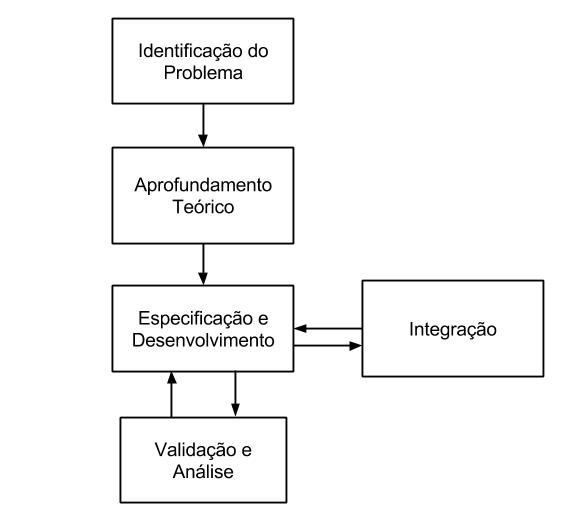
\includegraphics[scale=0.4]{figuras/metodologia.jpg}
\caption{Etapas da metodologia do projeto.} 
\label{fig:metodologia}
\end{figure}
\FloatBarrier

Na etapa inicial, definida como "Identificação do Problema", foi realizado um estudo do ambiente simulado 3D, através da 
especificação PEAS\cite{brussel} no domínio de futebol de robôs para identificar quais fatores influenciam na 
tomada de decisão do agente na identificação da melhor trajetória a ser seguida até o objetivo sem que haja colisão.

Na etapa seguinte, "Aprofundamento Teórico", foi realizado um estudo sobre planejamento de trajetória, planejamento multi-agente, 
coordenação multi-agente, predição de colisão e mapeamento de ambientes dinâmicos. Esta etapa teve como objetivo identificar 
trabalhos relacionados ao problema identificado na etapa anterior. O resultado do estudo foi descrito na Seção \ref{sec:trabalhosrelacionados}.

A etapa de "Especificação e Desenvolvimento" teve como base o desenvolvimento do modelo a partir da especificação dos requisitos e da 
modelagem da solução utilizando o time BahiaRT. Em conjunto com essa etapa, foi realizada a etapa de "Integração", fazendo as modificações 
necessárias no código do time BahiaRT e integrando o modelo desenvolvido.

Finalmente, na etapa "Validação e Análise", foi realizada uma especificação da metodologia de teste, da instalação do ambiente de teste e 
executados os testes para validar o modelo desenvolvido. Onde a validação foi realizada utilizando uma aplicação de passe 
desenvolvido para avaliar a eficácia das trajetórias encontradas, rodando o time com os melhores times da liga de simulação 3D dos últimos anos. E 
nesta mesma etapa, foram coletados os resultados obtidos, retornando a etapa anterior para corrigir falhas de desenvolvimento.

\section{Arquitetura do modelo}
\label{sec:arquitetura}
A arquitetura da aplicação de passe desenvolvida para validar o modelo proposto pode ser vista na figura \ref{fig:arquitetura}.

\begin{figure}[H]
\centering
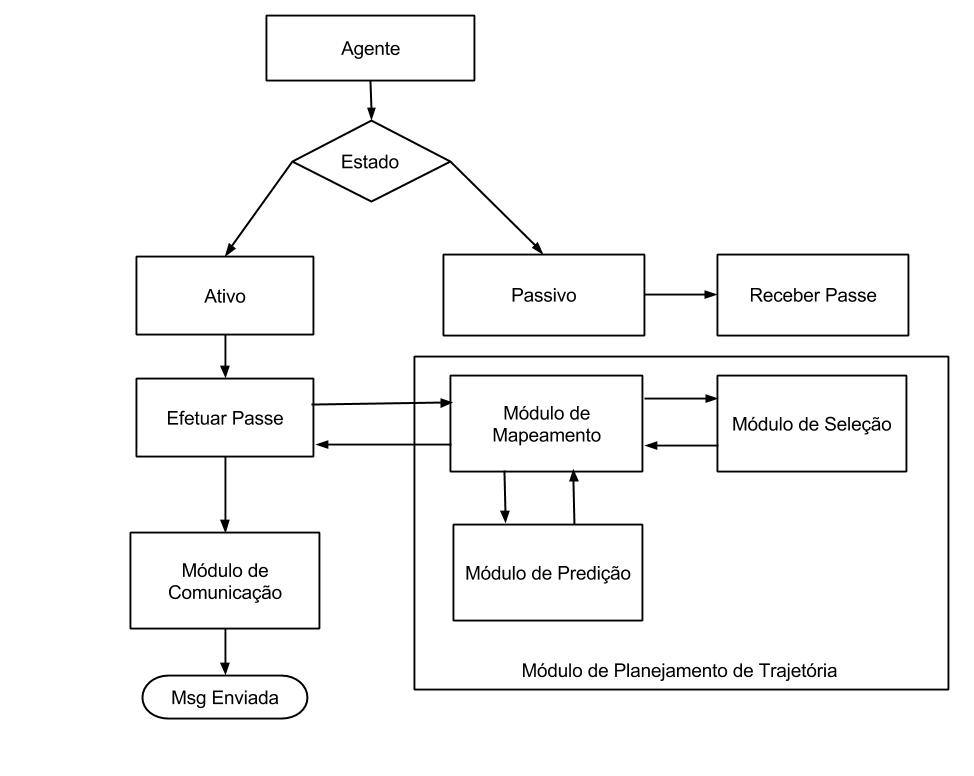
\includegraphics[scale=0.45]{figuras/ArquiteturaModelo.jpg}
\caption{Arquitetura do projeto desenvolvido integrado a um modelo de passe desenvolvido para validação.} 
\label{fig:arquitetura}
\end{figure}
\FloatBarrier

Nesta arquitetura, um agente pode estar em estavo ativo, ou passivo. Um agente em estado ativo, é designado como um agente que está com 
pose de bola, ou lutando pela pose de bola. Já os agentes passivos são considerados agentes de suporte, que ficam em posições estratégicas. No 
momento em que um agente está em estado ativo e com pose de bola, ele verifica a possibilidade de efetuar um passe.

O passe só é realizado se obedecer as seguintes regras:

\begin{enumerate}
 \item O oponente mais próximo deve estar a $4$ metros de distância.
 \item Deve existir pelo menos $1$ agente aliado em uma posição estratégica.
 \item O agente aliado que vai receber um passe não deve estar caído.
 \item O agente aliado que vai receber um passe não deve estar marcado por agentes oponentes.
 \item O agente que vai efetuar o passe deve estar em estado ativo e com a pose da bola.
 \item Deve existir uma trajetória confiável para onde o agente vai chutar a bola.
\end{enumerate}

Inicialmente é realizado o mapeamento e a busca das melhores trajetórias para lançar a bola. Depois é realizada uma busca dos melhores 
jogadores para receber o passe com base nas trajetórias. Em seguida o módulo de passe verifica dentre as trajetóris mapeadas e o 
posicionamento dos agentes aliados qual é a melhor trajetória para se obter sucesso no passe da bola. 

Quando a trajetória é escolhida, o agente envia uma mensagem {\it broadcast} avisando a posição em que a bola vai ser lançada e quem é o agente aliado que deve se deslocar para receber o passe. Quando os agentes recebem a mensagem, eles verificam se um passe está sendo realizado e quem é o agente escolhido 
para receber a bola. Por fim, o escolhido se deslocará para a posição estratégica que lhe foi comunicada.

O sucesso do passe depende não somente da aplicação desenvolvida, mas também do chute que vai ser realizado, levando em consideração os 
fatores tempo (tempo que o agente leva para chutar) e força (força aplicada pelo chute sobre a bola).

\section{Mapeamento das trajetórias}
\label{sec:map}
O mapeamento das trajetórias é realizado a partir da construção de um mapa de grade 2D, composto por células de tamanho igual 
que é projetado em segmentos em linhas $k$ do centro da trajetória. A construção do mapa leva em consideração as limitações do 
campo e o posicionamento do agente que vai calcular a melhor trajetória para alcançar o seu objetivo.

\begin{figure}[H]
\centering
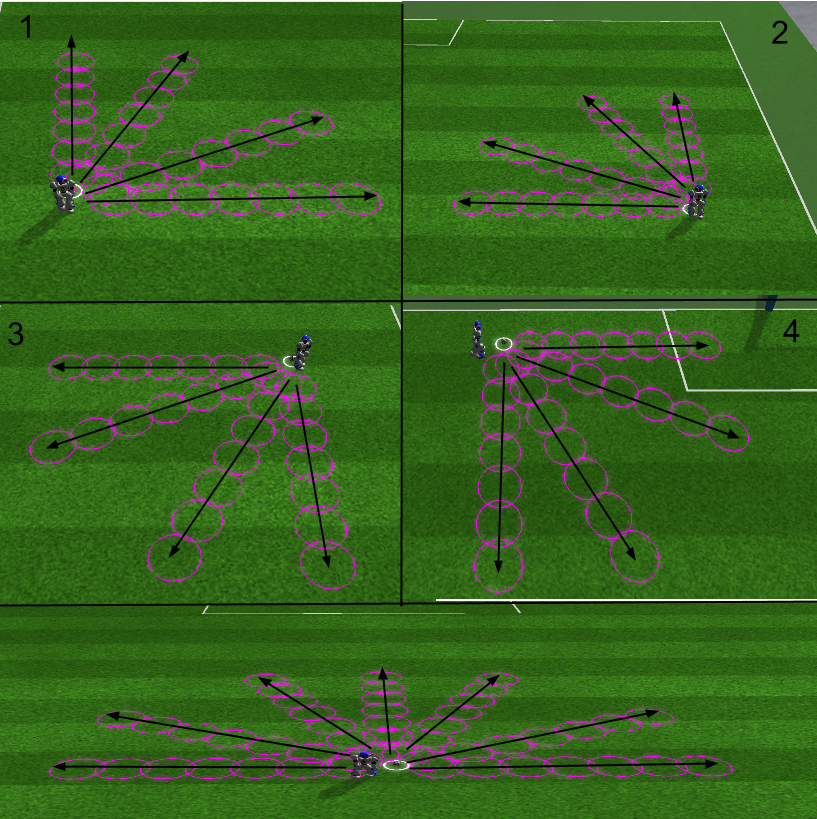
\includegraphics[scale=0.4]{figuras/Mapeamento.png}
\caption{Imagem do plot realizado pelo Roboviz representando os 5 tipos de mapeamento que é realizado pelo modelo desenvolvido.} 
\label{fig:mapeamento}
\end{figure}
\FloatBarrier

Para cada região do campo, foi definido um tipo de mapeamento, totalizando 5 tipos de mapeamento que são ilutrados na 
figura \ref{fig:mapeamento}. O objetivo foi evitar que regiões que não estavam dentro do campo fossem mapeadas e a quantidade
de células a serem verificadas fosse a menor possível, já que todo o processo de mapeamento e predição de trajetória deve ser 
feito em menos de $0.02$ segundos, que é o tempo de processamento mínimo do agente simulado 3D utilizado para desenvolvimento 
do modelo. 

Cada célula possui um conjunto de informações que são utilizadas no processo de predição da trajetória. No mapeamento de uma 
célula, apenas a posição e o número da célula são armazenados, sendo que o número representa a trajetória. As outras informações
da célula são incluídas no processo de verificação da presença de obstáculos que será descrito na próxima seção.

O diagrama de classe da célula pode ser visto na figura \ref{fig:celula}.

\begin{figure}[!htb]
\centering
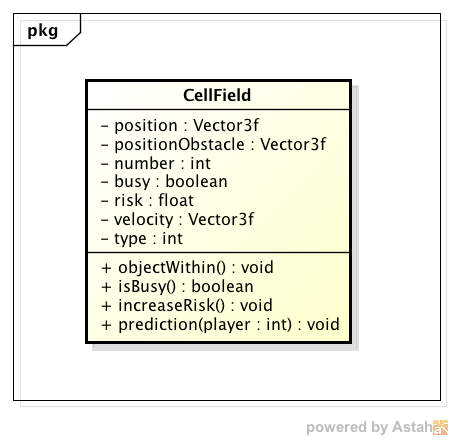
\includegraphics[scale=0.8]{figuras/celula.png}
\caption{Diagrama da classe CellFied utilizado no modelo para representar uma únidade do mapeamento.}
\label{fig:celula}
\end{figure}
\FloatBarrier

\section{Verificação da presença de obstáculos}
\label{sec:verifobstaculos}
A verificação da presença de obstáculos é feita logo após o processo de mapeamento das trajetórias. O modelo levou em consideração 
que os agentes aliados não são considerados obstáculos por conta do processo de coordenação e planejamento multi-agente que é 
realizado através do protocolo de comunicação utilizado pelo BahiaRT. Neste processo de coordenação, quando o agente encontrar a 
melhor trajetória, ele enviará uma mensagem através do canal de comunicação para todos os agentes aliados, informando a trajetória e 
outras informações que fazem parte do seu estado de mundo. O objetivo é atualizar todos os agentes sobre o estado atual do 
agente ativo.

\begin{algorithm}[!htb]
\caption{Algoritmo para verificação da presença de obstáculos}

\begin{algorithmic}[3.1]
\For{k}{1}{n}
  \For{i}{2}{11}
  
  \State $map[k].prediction(agent[i])$ \Comment{Realiza a predição de colisão}
  
  \If {$!map[k].isBusy()$}
    
    \If {$map[k].objectWithin(agent[i].position)$}
     \If {$agente[i].conf > minReliability $}
     
     \State {$map[k].velocity \gets  agent[i].velocity$} \Comment{Armazena a velocidade}
     \State {$map[k].positionOB \gets  agent[i].position$} \Comment{Armazena a posição}
     \State {$map[k].type \gets  OPPONENT$} \Comment{Armazena o tipo de obstáculo}
     \State {$map[k].busy \gets  true$} \Comment{Define a célula como ocupada}
     \State {$map[k].IncreaseRisk()$} \Comment{Incrementa o risco}
     
     \EndIf
    \EndIf
  \EndIf
  \EndFor
\EndFor
\end{algorithmic}
\end{algorithm}

No processo de verificação da presença de obstáculos, algoritmo 1, se uma célula estiver ocupada por um 
obstáculo, as informações desse obstáculo serão armazenadas. Neste processo, a posição do obstáculo, a velocidade e o tipo 
de obstáculo são armazenados na célula. Como neste domínio, apenas os agentes oponentes são considerados obstáculos, só 
existirão obstáculos de um tipo, que são os oponentes. Além dessas informações, uma taxa que indica o risco da célula é 
incrementada para indicar posteriormente se a trajetória é viável.

Cada agente possui informações dos oponentes que são utilizadas para verificar a presença dos obstáculos. Estas informações 
possuem uma taxa de confiabilidade que representa o quanto essas informações estão atualizadas. Neste processo de verificação, 
apenas os agentes oponentes que possuem no mínimo $80\%$ de confiabilidade são levados em consideração.

%\section{Calculo da velocidade dos obstáculos}
\section{Determinação da trajetória de objetos dinâmicos em ambientes ruidosos}
\label{sec:calcvel}

Para calcular a velocidade e direção dos obstáculos foi desenvolvido um modelo que filtra o ruído posicional (oscilações fortes da posição 
do objeto visto em torno da sua trajetória real) e calcula a velocidade vetorial e a escalar do objeto com poucas oscilações.

Para isso, um vetor é estendido desde a posição filtrada em cada ciclo, para o futuro, para predizer a posição futura do objeto.
Ao invés de calcular a média das velocidades, foi utilizado uma função que utiliza mínimos quadrados \cite{minQuad} 
para encontrar um valor coerente com o movimento do objeto.

Seja $n$ uma sequencia ordenada de $N$ valores numericos $n_{i},\: i=1,2,\ldots,N$.
Denotodo por $S_{a,b}(n)$ o operador que extrai uma subsequência $s=\{n_{a},n_{a+1},\ldots,n_{b-1},n_{b}\}$
da sequência $n$, sempre que $a\leq b$. Sejam $x_{i}$ e $y_{i}$
as coordenadas medidas de um objeto rastreado num plano no instante
$t_{i},\: i\geq0$. A figura \ref{fig:Sequ=0000EAncia-de-pontos-medidos}
demonstra uma sequência de pontos medidos de um objeto monitorado
pelo agente no campo de futebol, que foi localizado quando estava
parado na esquerda do gráfico e começou a se movimetar para a direita
fazendo uma trajetória complexa, que inclui um giro de $360$ graus.

\begin{figure}[!htb]
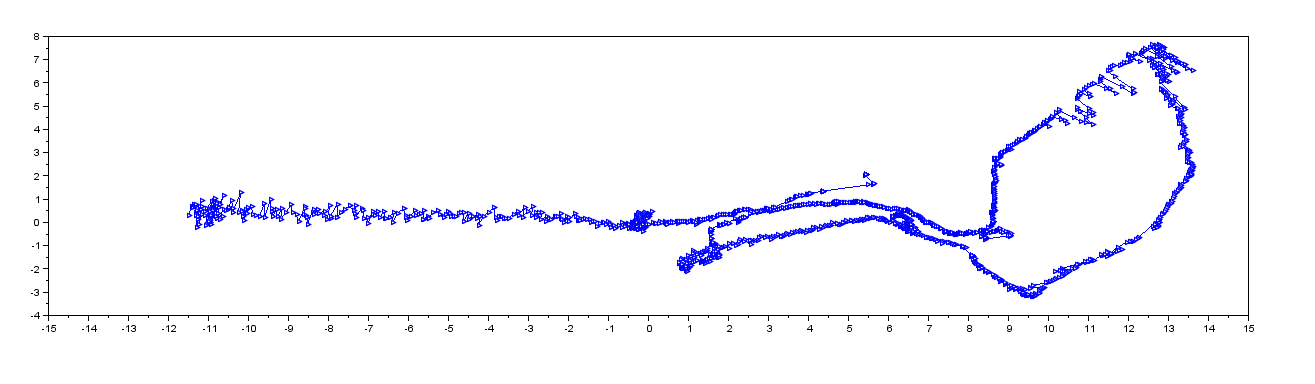
\includegraphics[scale=0.45]{figuras/fig_pontos_medidos}
\caption{\label{fig:Sequ=0000EAncia-de-pontos-medidos}Sequência de pontos
medidos de um objeto monitorado pelo agente no campo de futebol }
\end{figure}

Vale notar que independentemente do sistema sensorial utilizado, existirá
uma diferença entre o ponto medido $p_{i}=(x_{i},y_{i})$ e o ponto
onde realmente se encontra o objeto rastreado nesse instante $P_{i}=(X_{i},Y_{i})$.
Em ambientes simulados é possível realizar experimentos e registrar as
posições reais do alvo em intervalos de tempo discretos $t_{k}$ para
$k=1,2,\ldots,i$, isto é, coletando a trajetória real e medida
através de séries temporais $P=\left\{ P_{1},P_{2},\ldots,P_{i}\right\} $
e $p=\left\{ p_{1},p{}_{2},\ldots,p_{i}\right\} $. A figura \ref{fig:pontossemfiltro}
demonstra o resultado obtido em um dos experimentos, onde o objeto
foi localizado na esquerda do gráfico e começou a se movimentar para
a direita. A cor vermelha representa os pontos reais e a cor
azul os ponto medidos. 

\begin{figure}[!htb]
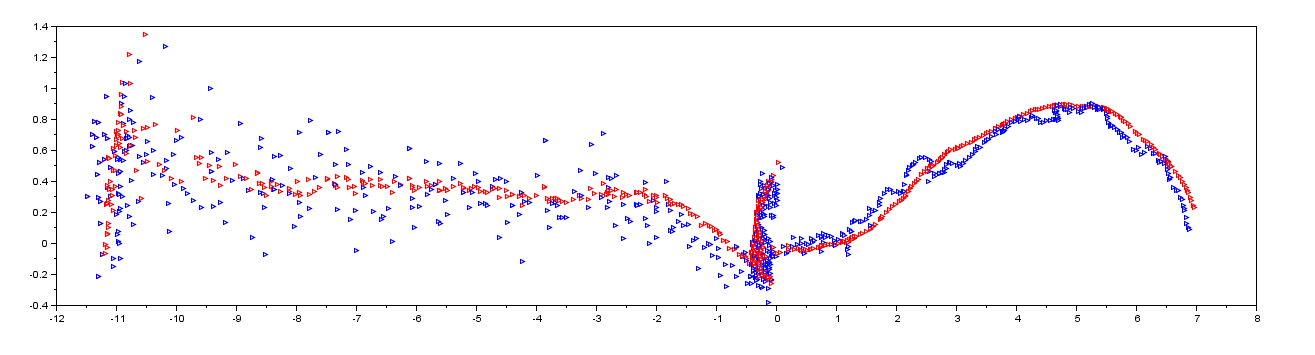
\includegraphics[scale=0.45]{figuras/fig_pontos_medidos_e_reais}
\caption{Sequência de pontos medidos e estimados de um objeto monitorado pelo agente
no campo de futebol }
\label{fig:pontossemfiltro}
\end{figure}


Note que a distância entre a posição medida $p_{i}$ e a posição real
$P_{i}$ do objeto, resultado do ruído inerente do sistema de medição,
varia com o tempo o que indica que o sistema sensorial em teste é
autoajustado, mas que mesmo assim nunca desaparece. A intensidade
do ruído posicional instantâneo vem dada por $r_{i}=\left\Vert p_{i}-P_{i}\right\Vert $
onde o operador $\left\Vert \cdot\right\Vert $ representa a norma
euclideana do vetor argumento.

Desde o ponto de vista de filtragem de ruído, o resultado relevante
são os últimos $u$ instantes da trajetória, designados como trajetórias
recentes no instante $i$, e denotados por $\Pi_{i}=S_{i-u,i}(P)=\left\{ P_{i-u},P_{i-u+1},\ldots,P_{i-1},P_{i}\right\} $
e $\pi_{i}=S_{i-u,i}(p)=\left\{ p_{i-u},p_{i-u+1},\ldots,p_{i-1},p_{i}\right\} $. 

Considerando que qualquer trajetória pode ser aproximada por uma sucessão
de segmentos de trajetórias lineares, foi utilizado o método dos
mínimos quadrados para estimar uma aproximaçao mais confiável $\tilde{P}_{i}$
da posição real do alvo no instante $i$, e com isto poder estimar
sua direção e velocidade absoluta utilizando um ponto estimado no
passado $\tilde{P}_{i-lag}$, com $lag\geq1$. A hipótese principal
do estudo é a base provada do método dos mínimos quadrados segundo
o qual $\left\Vert p_{i}-P_{i}\right\Vert \geq\left\Vert \tilde{P}_{i}-P_{i}\right\Vert $,
em média \cite{minQuad}. 

O procedimento utilizado foi o seguinte:
\begin{enumerate}
\item Obter a posição filtrada $\tilde{P}_{i}$ através de duplo ajuste
com mínimos quadrados supondo os resultados com as primeiras derivadas
das funções obtidas em cada ajuste, isto é

\begin{enumerate}
\item Cálculo dos coeficientes $a_{xy},b_{xy}$ da reta $y=a_{xy}+b_{xy}x$,
utilizando mínimos quadrados com os últimos $u-1$ pontos filtrados
$\left(\tilde{x}_{j},\tilde{y}_{j}\right),\: j=i-u,\ldots i-1$ e
o ponto medido$\left(x_{i},y_{i}\right)$. 
\item Cálculo dos coeficientes $a_{yx},b_{yx}$ da reta $x=a_{yx}+b_{yx}y$,
utilizando mínimos quadrados com os últimos $u-1$ pontos filtrados
$\left(\tilde{y}_{j},\tilde{x}_{j}\right),\: j=i-u,\ldots i-1$ e
o ponto medido $\left(y_{i},x_{i}\right)$.
\item Cálculo de dois pontos no presente (instante $i$) , $p_{1,i}=\left(x_{1,i},y_{1,i}\right)$
e $p_{2,i}=\left(x_{2,i},y_{2,i}\right)$, da forma
\[
x_{1,i}=x_{i}
\]
\[
y_{1,i}=a_{yx}+b_{yx}x_{i}
\]
\[
x_{2,i}=a_{xy}+b_{xy}y_{i}
\]
\[
y_{2,i}=y_{i}
\]

\item Cálculo do ponto mais provável no presente (instante $i$) $\tilde{P}_{i}=\left(\tilde{x}_{i},\tilde{y}_{i}\right)$
a partir dos 2 pontos acima, utilizando como peso a primeira derivada,
da forma
\[
\tilde{P}_{i}=\left(\frac{1}{b_{xy}+b_{yx}}\right)\left(b_{yx}p_{1,i}+b_{xy}p_{2,i}\right)
\]

\end{enumerate}
\item Obter a direção de movimento mais provável e a velocidade absoluta
do objeto utilizando novamente mínimos quadrados e diferenças finitas,
isto é

\begin{enumerate}
\item Cálculo dos coeficientes $a_{xy},b_{xy}$ da reta $y=a_{xy}+b_{xy}x$,
utilizando mínimos quadrados com os últimos $u$ pontos filtrados
$\left(\tilde{x}_{j},\tilde{y}_{j}\right),\: j=i-lag,\ldots i$. 
\item Cálculo dos coeficientes $a_{yx},b_{yx}$ da reta $x=a_{yx}+b_{yx}y$,
utilizando mínimos quadrados com os últimos $u$ pontos filtrados
$\left(\tilde{y}_{j},\tilde{x}_{j}\right),\: j=i-lag,\ldots i$.
\item Cálculo de dois pontos no passado (instante $i-lag+1$) , $p_{1,i-lag+1}=\left(x_{1,i-lag+1},y_{1,i-lag+1}\right)$
e $p_{2,i-lag+1}=\left(x_{2,i-lag+1},y_{2,i-lag+1}\right)$, da forma
\[
x_{1,i-lag+1}=\tilde{x}_{i-lag+1}
\]
\[
y{}_{1,i-lag+1}=a_{yx}+b_{yx}x_{1,i-lag+1}
\]
\[
y_{2,i-lag+1}=\tilde{y}_{i-lag+1}
\]
\[
x_{2,i-lag+1}=a_{xy}+b_{xy}y_{2,i-lag+1}
\]

\item Cálculo do ponto médio no passado (instante $i-lag+1$) $\hat{P}_{i-lag+1}$
a partir dos 2 pontos no passado calculados acima, isto é,
\[
\hat{P}_{i-lag+1}=0.5\left(p_{1,i-lag+1}+p_{2,i-lag+1}\right)
\]

\item Cálculo de dois pontos no presente (instante $i$) , $p_{1,i}=\left(x_{1,i},y_{1,i}\right)$
e $p_{2,i}=\left(x_{2,i},y_{2,i}\right)$, da forma
\[
x_{1,i}=\tilde{x}_{i}
\]
\[
y{}_{1,i}=a_{yx}+b_{yx}x_{1,i}
\]
\[
y_{2,i}=\tilde{y}_{i}
\]
\[
x_{2,i}=a_{xy}+b_{xy}y_{2,i}
\]

\item Cálculo do ponto médio no presente (instante $i$) $\hat{P}_{i}$
a partir dos 2 pontos no presente calculados acima, isto é,
\[
\hat{P}_{i}=0.5\left(p_{1,i}+p_{2,i}\right)
\]

\item Cálculo do vetor velocidade no presente (instante $i$), $v_{i}=\left(v_{x,i},v_{y,i}\right)$,
tal 
\[
v_{i}=\frac{\hat{P}_{i}-\hat{P}_{i-lag+1}}{t_{i}-t_{i-lag+1}}
\]

\item Cálculo da velocidade escalar no presente (instante $i$), $V_{i}=\left\Vert v_{i}\right\Vert $.
\item Cálculo do vetor de direçao no presente (instante $i$), $d_{i}={\displaystyle \frac{1}{\left\Vert v_{i}\right\Vert }}v_{i}$.\end{enumerate}
\end{enumerate}


Com o algoritmo para filtrar o ruído posicional e calcular a velocidade vetorial e escalar do agente, foi possível estimar os 
pontos de colisão com maior precisão, auxiliando na escolha da melhor trajetória.

\section{Predição de colisão dos obstáculos}
\label{sec:calctrajetoria}
Neste modelo, além de levar em consideração a presença de obstáculos nas trajetórias, é realizado um processo de predição de 
deslocamento dos obstáculos que estão em regiões próximas com o objetivo de predizer se o obstáculo irá estar na trajetória 
no mesmo instante em que o agente estiver se deslocando para o ponto objetivo, ou se tiver chutado a bola na trajetória escolhida 
e ela estiver se deslocando até o ponto objetivo.

O principal objetivo da predição é evitar que o agente ou a bola colida com o obstáculo no momento em que estiver se deslocando 
em direção ao objetivo. A partir desta análise, se um agente oponente levar um tempo menor para chegar ao ponto $P$ da trajetória, 
que o agente aliado, ou a bola, então o risco deste ponto aumenta, sendo que cada ponto é considerado como a célula da trajetória, 
e que para cada célula, são verificados os agentes oponentes próximos desta trajetória que foi mapeada.

O calculo da predição do deslocamento do agente oponente é realizado com a velocidade do agente calculada e a distância entre o 
oponente e a trajetória:

\begin{equation}
D = A - B 
\end{equation}
\begin{equation}
T = \frac {D} {V}
\end{equation}

onde $D$ é a distância do ponto $A$ ao ponto $B$, $V$ é a velocidade do oponente e $T$ é o tempo que o agente
levaria até chegar ao ponto $B$, levando em consideração que a velocidade é constante.

O cálculo do ponto previsto é descrito como:

\begin{equation}
  P = Po + V * T 
\end{equation}

onde $P$ é o ponto previsto, $Po$ é a posição atual, $V$ é a velocidade e $T$ é o tempo em que estou estimando a posição. O 
algoritmo resumido pode ser visto abaixo no algoritmo 2.

\begin{algorithm}[!htb]
\label{alg:prediction}
\caption{Algoritmo para predição de colisão}
\begin{algorithmic}[3.2]
\Function{Prediction}{agent}
  \If {$agent.conf < minReliability$}
    \State \Return
  \EndIf
  
  \State {$ballTime \gets distanceBallToCellField / velBall$}
  \State {$meTime \gets distanceMeToCellField / velMe$}
  \State {$deltaS \gets agent.distanceToCellField$}
  \State {$agentSpeed \gets agent.velocity$}
  
  \If {$agentSpeed <= 0 $}
    \State $agentSpeed \gets 0.1$
  \EndIf
  
  \State {$deltaT \gets deltaS / agentSpeed$}
  \State {$estimedPostition \gets agent.position + agent.velocity * deltaT$}
  
  \If{$objectWithin(estimedPostition)$}
  
    \If{$((deltaT+TIME_PERCEPTION) < ballTime) || (deltaT+TIME_PERCEPTION < meTime)$}
      \State $increaseRisk()$
    \EndIf
    
    
    \If {$(maxVelocityAgent - agentSpeed) < minVel$}
      \State $increaseRisk()$
      \State $increaseRisk()$
    \Else
      \State $increaseRisk()$
    \EndIf
    
  \EndIf
\EndFunction
\end{algorithmic}
\end{algorithm}

\section{Critério do descarte de obstáculos}
\label{sec:descarte}
O modelo levou em consideração apenas os obstáculos que possuíam informações atualizadas e que estavam próximos da trajetória. O 
objetivo foi evitar utilizar obstáculos que não possuem nenhum risco para a predição da trajetória.

    
